% Test deck. Build: python presentation/make_frames.py, then pdflatex main.tex (in presentation/).
% The animation plays in Acrobat / Okular; other viewers show the first frame.
\documentclass[aspectratio=169]{beamer}
\usetheme{default}
\setbeamertemplate{navigation symbols}{}
\setbeamertemplate{footline}[frame number]
\usepackage{animate}
\usepackage{amsmath,amssymb}
\usepackage{booktabs}
\definecolor{Ecol}{HTML}{1F8AD0}  % Song 2016 Fig. 1 colours: E blue, I red
\definecolor{Icol}{HTML}{E0393E}

\title{Multitask Dale's-law RNNs under metabolic and wiring budgets}
\author{Atharv Suryawanshi}
\institute{Msc Neuroscience, GSN}
\date{\today}

\begin{document}

\begin{frame}
  \titlepage
\end{frame}

\begin{frame}{One circuit, many tasks}
  \centering
  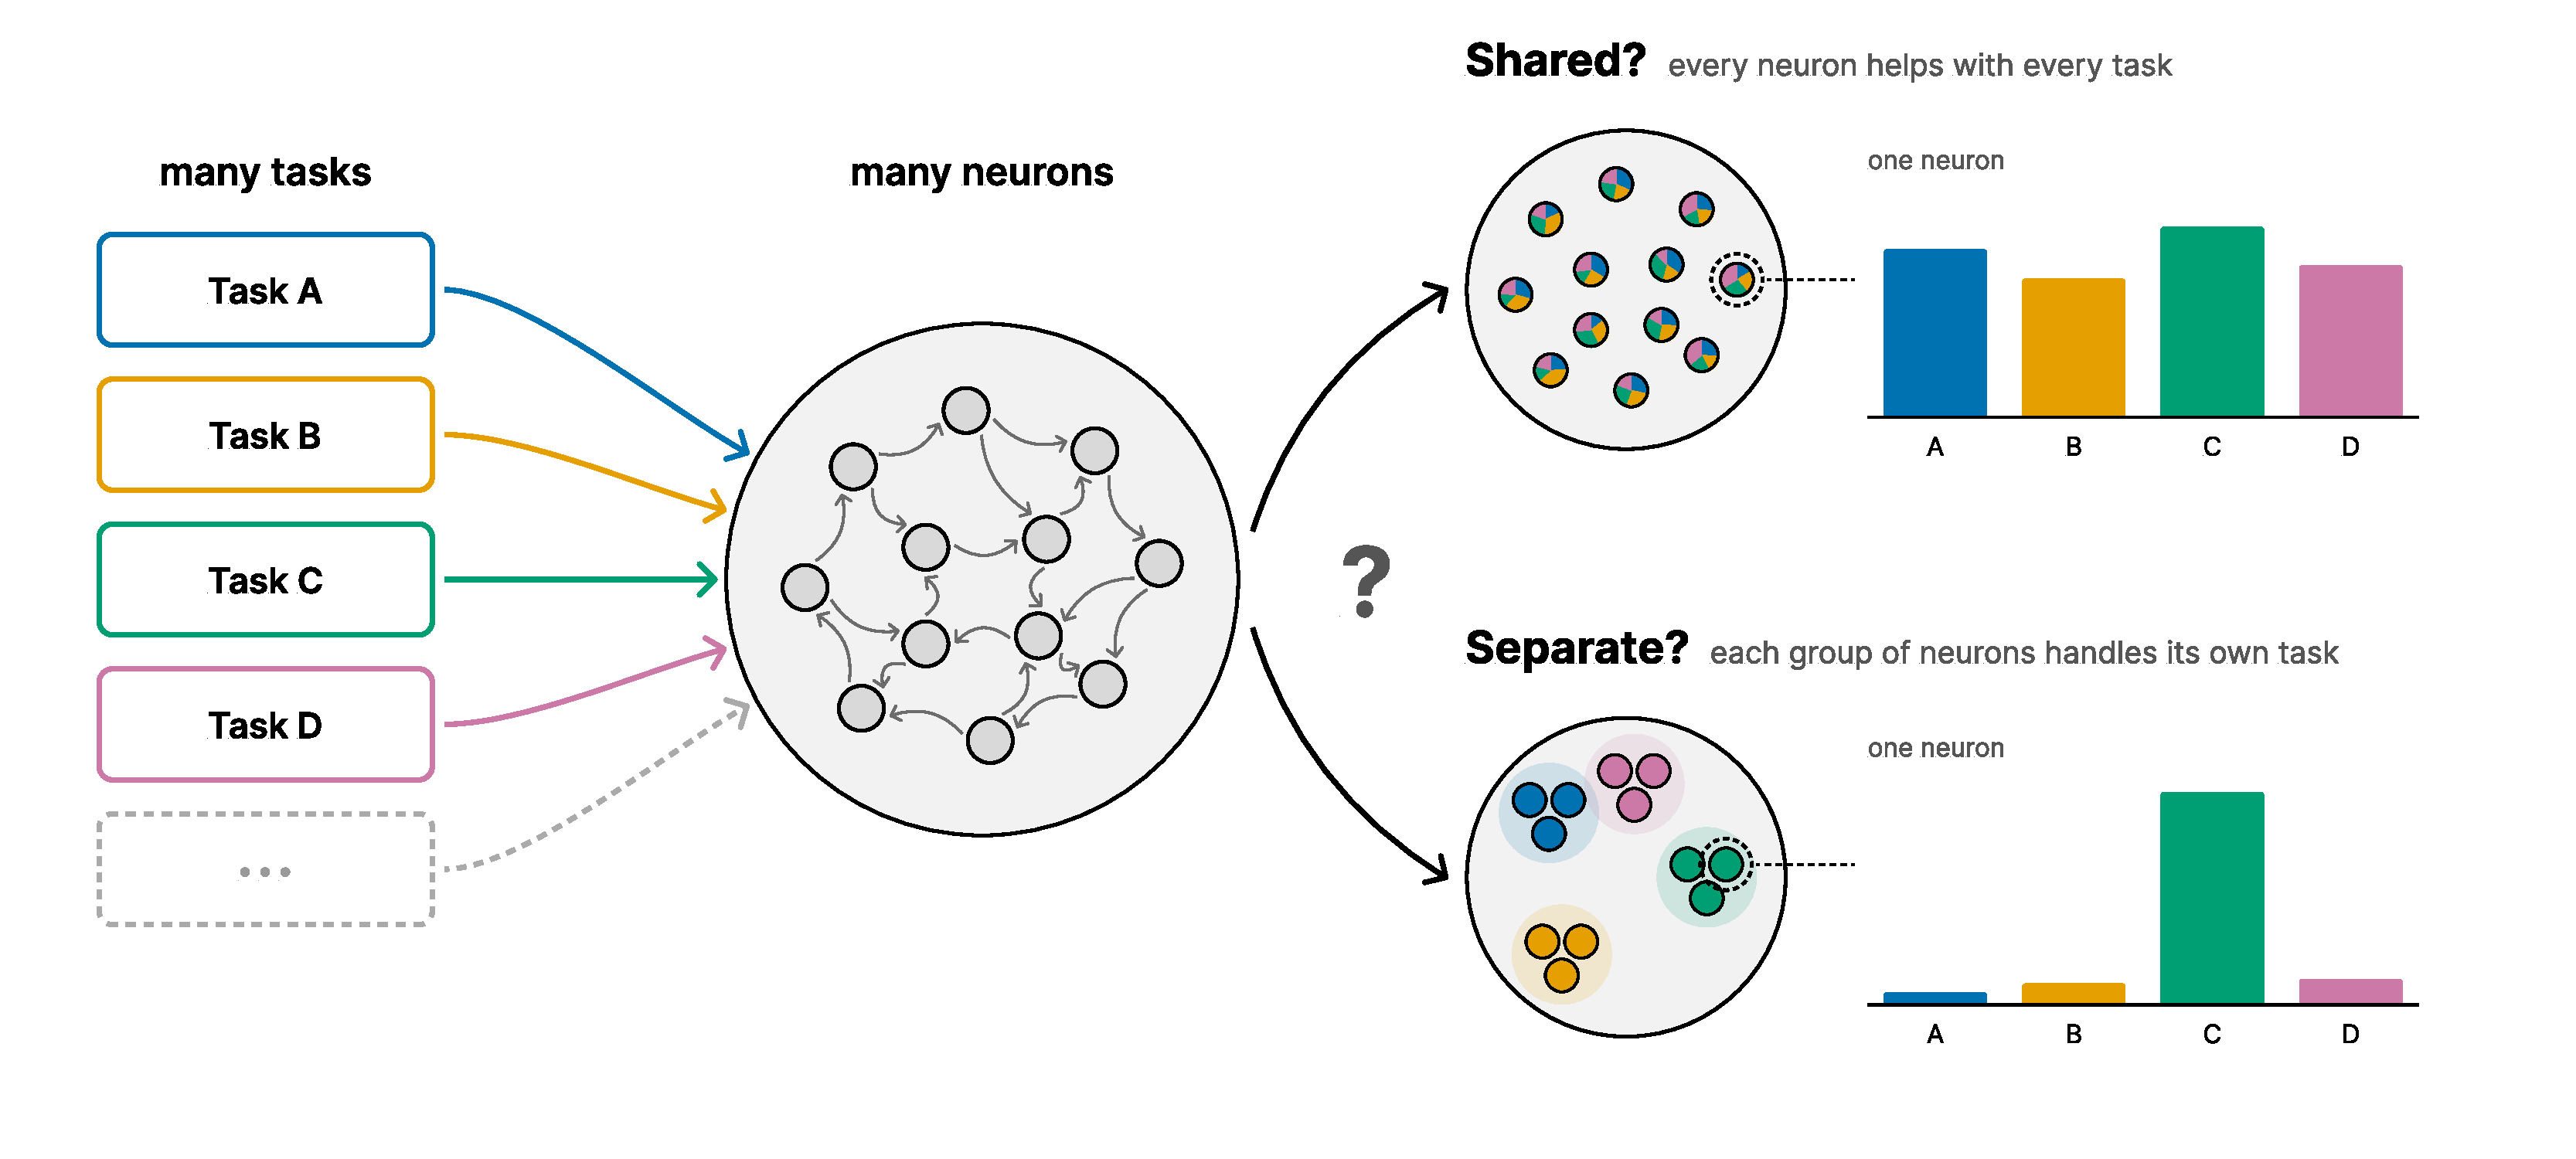
\includegraphics[width=\textwidth,height=0.82\textheight,keepaspectratio]{figs/fig1_intro_question.pdf}
\end{frame}

\begin{frame}{Yang et al.\ 2019: one network, 20 tasks}
  \begin{columns}[T]
    \begin{column}{0.48\textwidth}
      \centering
      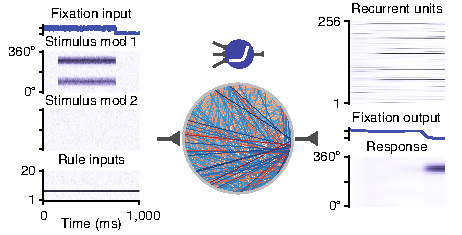
\includegraphics[width=\linewidth,page=1]{figs/yang2019_crops.pdf}\\[0.8em]
      \footnotesize 256 Vanilla RNNs trained on 20 cognitive tasks at once:
      fixation, two stimulus rings and a rule input in; fixation and a response ring out.
    \end{column}
    \begin{column}{0.48\textwidth}
      \centering
      \includegraphics[width=\linewidth,page=2]{figs/yang2019_crops.pdf}\\[0.8em]
      \footnotesize Task variance: how much each neuron takes part in each task.
      Neurons form clusters, each specialised for a group of related tasks.
    \end{column}
  \end{columns}
  \vfill
  {\scriptsize Yang, Joglekar, Song, Newsome \& Wang (2019). Task representations in neural networks trained to
  perform many cognitive tasks. \emph{Nat.\ Neurosci.} 22, 297--306. Figs 1b, 2a--c.}
\end{frame}

\begin{frame}{Song, Yang \& Wang 2016: excitatory and inhibitory neurons}
  \begin{columns}[c]
    \begin{column}{0.5\textwidth}
      \centering
      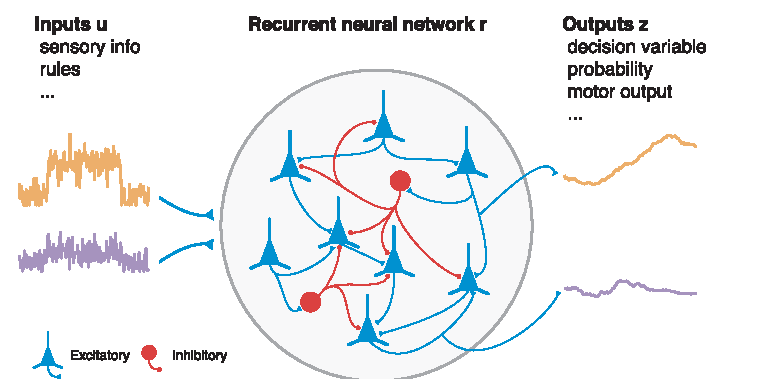
\includegraphics[width=\linewidth]{figs/song2016_crops.pdf}
    \end{column}
    \begin{column}{0.48\textwidth}
      \small
      \begin{align*}
        \tau\dot{\mathbf{x}} &= -\mathbf{x} + W^{\mathrm{rec}}\mathbf{r} + W^{\mathrm{in}}\mathbf{u} + \text{noise}\\
        \mathbf{r} &= [\mathbf{x}]_+, \qquad \mathbf{z} = W^{\mathrm{out}}\,\mathbf{r}_{\textcolor{Ecol}{\mathrm{E}}}\\[0.4em]
        W^{\mathrm{rec}} &= W^{\mathrm{rec},+}\,D, \qquad W^{\mathrm{rec},+} \geq 0\\
        D &= \mathrm{diag}(\underbrace{\textcolor{Ecol}{+1,\dots,+1}}_{\text{E}},\
                           \underbrace{\textcolor{Icol}{-1,\dots,-1}}_{\text{I}})
      \end{align*}
      \footnotesize
      \begin{itemize}
        \item Dale's law: each neuron is \textcolor{Ecol}{excitatory} or \textcolor{Icol}{inhibitory}
              (80\,/\,20); the sign of its outgoing synapses is fixed.
        \item One network per task (decision making, working memory, \dots); activity resembles recordings.
      \end{itemize}
    \end{column}
  \end{columns}
  \vfill
  {\scriptsize Song, Yang \& Wang (2016). Training excitatory-inhibitory recurrent neural networks for cognitive
  tasks: a simple and flexible framework. \emph{PLoS Comput.\ Biol.} 12(2), e1004792. Fig.~1, Eqs 1--3, 12.}
\end{frame}

\begin{frame}{Real neurons pay for firing and for wiring}
  \vfill
  \begin{itemize}\setlength{\itemsep}{1.4em}
    \item \textbf{Firing costs energy.} Spikes and synaptic transmission dominate the brain's energy budget,
          so activity has to be sparse.\\
          {\scriptsize\color{gray} Attwell \& Laughlin 2001; Lennie 2003}
    \item \textbf{Wiring costs space.} Axons and dendrites fill most of the grey matter,
          so connections have to be few.\\
          {\scriptsize\color{gray} Chklovskii, Schikorski \& Stevens 2002}
    \item \textbf{\dots and the circuit must still solve its tasks.}
  \end{itemize}
  \vfill
\end{frame}

\begin{frame}{Setup}
  \centering
  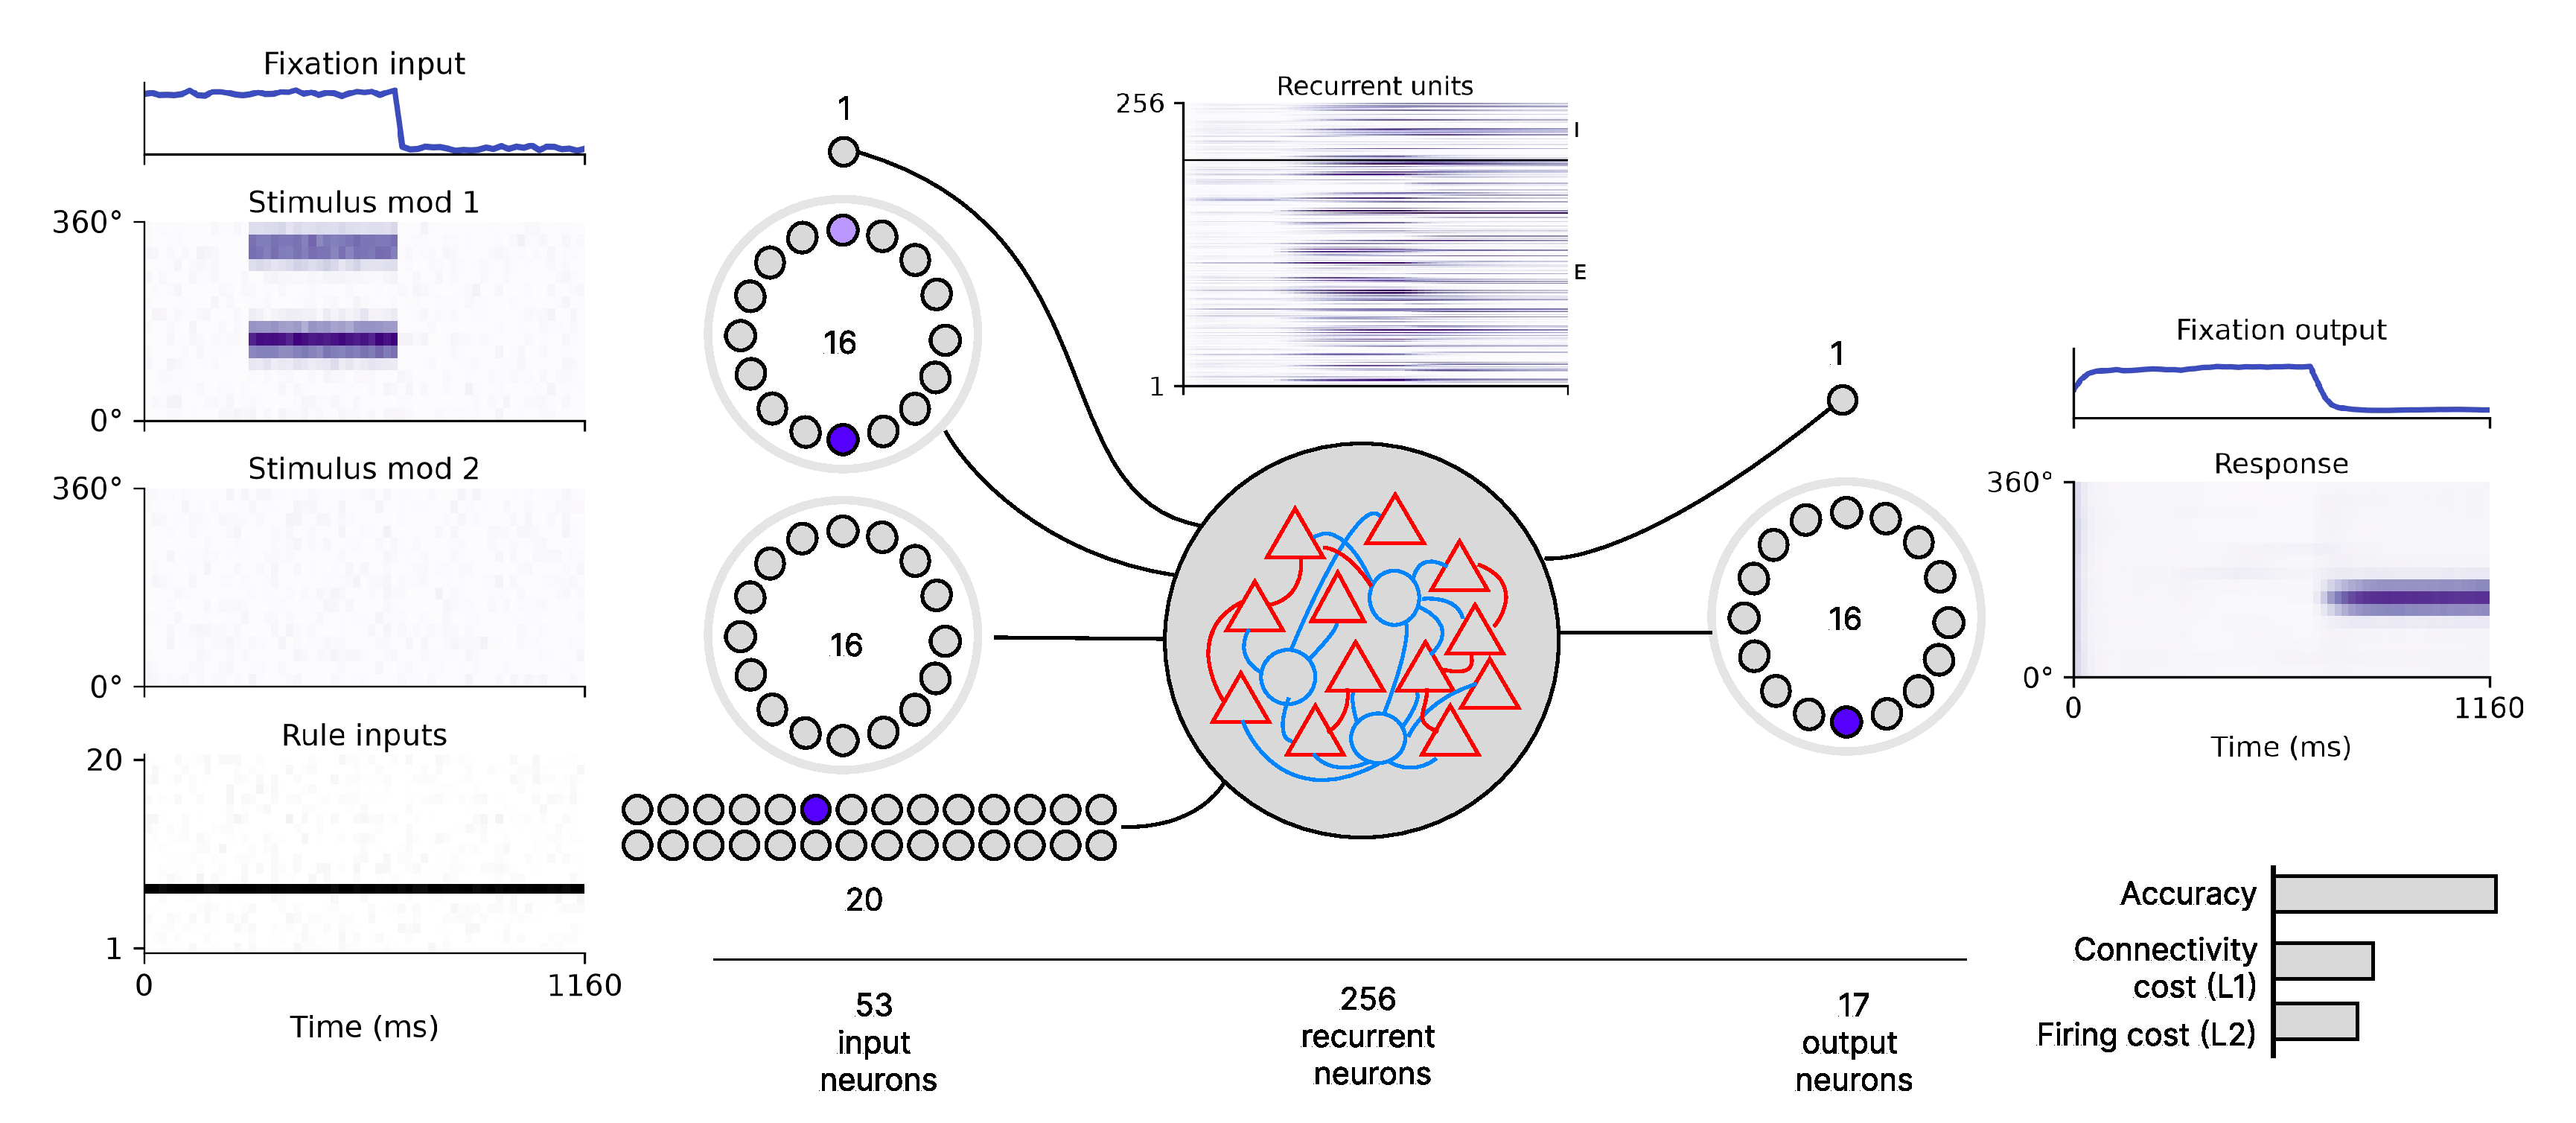
\includegraphics[width=\textwidth]{figs/fig_setup.pdf}\\[0.8em]
  \small 256 rate neurons (204 E, 52 I), all 20 Yang tasks trained together in one network, 150k steps.
\end{frame}

\begin{frame}{The network}
  \small
  \begin{align*}
    \mathbf{r}_t &= (1-\alpha)\,\mathbf{r}_{t-1}
       + \alpha\,\big[\,W^{\mathrm{in}}\mathbf{u}_t + W^{\mathrm{rec}}\mathbf{r}_{t-1} + \mathbf{b} + \sigma\boldsymbol{\xi}_t\,\big]_+,
       \qquad \alpha = \Delta t/\tau = 20\,\text{ms}/100\,\text{ms}\\[0.6em]
    W^{\mathrm{rec}} &= \big(\mathrm{softplus}(\Theta)\odot(\mathbf{1}-I)\big)\,D,
       \qquad D = \mathrm{diag}(\underbrace{\textcolor{Ecol}{+1,\dots,+1}}_{204\ \text{E}},\
                                \underbrace{\textcolor{Icol}{-1,\dots,-1}}_{52\ \text{I}})\\[0.6em]
    \hat{\mathbf{y}}_t &= \mathrm{sigmoid}\big(W^{\mathrm{out}}\,\mathbf{r}^{\textcolor{Ecol}{\mathrm{E}}}_t + \mathbf{b}^{\mathrm{out}}\big)
  \end{align*}
  \vspace{0.4em}
  \footnotesize
  \begin{itemize}
    \item $\mathrm{softplus}(\Theta) \geq 0$: learned synaptic strengths. $D$: fixed sign of each presynaptic neuron (Dale).
          $\mathbf{1}-I$: no autapses.
    \item Readout from E neurons only. $W^{\mathrm{in}}$, $W^{\mathrm{rec}}$, $W^{\mathrm{out}}$ all trained.
    \item Adam, learning rate $10^{-3}$, batch 32, 150k steps; spectral radius of $W^{\mathrm{rec}}$ set to 1 at init.
  \end{itemize}
\end{frame}

\begin{frame}{Three objectives}
  \small
  \begin{align*}
    \text{Task:}\quad L_{\text{task}} &= \Big\langle \frac{\sum_{t,k} m_{tk}\,(\hat y_{tk} - y_{tk})^2}{\sum_{t,k} m_{tk}} \Big\rangle_{\text{trials}}\\[0.6em]
    \text{Firing:}\quad C_{\text{fire}} &= \big\langle\, r_i(t)^2 \,\big\rangle_{\text{trials},\,t,\,i}\\[0.6em]
    \text{Wiring:}\quad C_{\text{wire}} &= \frac{1}{N(N-1)} \sum_{i \neq j} \frac{|W^{\mathrm{rec}}_{ij}|}{c_j},
      \qquad c_j = \begin{cases} 1 & j \in \textcolor{Ecol}{\text{E}}\\ n_{\text{E}}/n_{\text{I}} & j \in \textcolor{Icol}{\text{I}} \end{cases}
  \end{align*}
  \vspace{0.4em}
  \footnotesize
  \begin{itemize}
    \item Task: squared error where the target matters ($m$), each trial weighted equally.
    \item Firing: mean squared rate over trials, time and neurons.
    \item Wiring: L1 of the recurrent weights, which pushes weak synapses to zero (fewer connections).
          $c_j$ divides out the $\sim$4$\times$ stronger I synapses, so inhibition is not pruned first.
  \end{itemize}
\end{frame}

\begin{frame}{Holding the network to a budget}
  \begin{columns}[T]
    \begin{column}{0.48\textwidth}
      \textbf{Wiring: hard limit}\\[0.3em]
      \footnotesize Not in the loss. After every Adam step, all synapses shrink by the same amount
      until the cost fits; weak synapses reach zero (projection onto the L1 ball).
      \small
      \[
        |W_{ij}| \leftarrow \max\big(|W_{ij}| - \theta,\ 0\big),\quad
        \theta:\ C_{\text{wire}} = B_{\text{wire}}
      \]
    \end{column}
    \begin{column}{0.48\textwidth}
      \textbf{Firing: soft limit}\\[0.3em]
      \footnotesize Activity cannot be clipped, so it is penalised with a weight $\lambda$ that tunes itself:
      up while over budget, down while under.
      \small
      \begin{align*}
        L &= L_{\text{task}} + \lambda\,C_{\text{fire}} + \tfrac{\rho}{2}\,B_{\text{fire}}\big[\tfrac{C_{\text{fire}}}{B_{\text{fire}}} - 1\big]_+^2\\
        \log\lambda &\leftarrow \log\lambda + \eta\,\big(\tfrac{C_{\text{fire}}}{B_{\text{fire}}} - 1\big)
      \end{align*}
    \end{column}
  \end{columns}
  \vfill
  \footnotesize No hand-set trade-off weights: each network gets two ceilings, $(B_{\text{fire}}, B_{\text{wire}})$,
  and is trained to be as accurate as possible under them.
  \vfill
  {\scriptsize\color{gray} L1 projection: Duchi et al.\ 2008.}
\end{frame}

\begin{frame}{Mapping the front: NSGA-III (pymoo)}
  \small
  \begin{itemize}\setlength{\itemsep}{0.6em}
    \item \textbf{Minimise} \ $\big(1 - \text{worst-task accuracy},\ \log C_{\text{fire}},\ \log C_{\text{wire}}\big)$,
          \ subject to worst-task accuracy $\geq 0.6$.
    \item \textbf{Pareto front}: networks where no objective can improve without another getting worse.
    \item \textbf{Two nested loops}: NSGA-III chooses the budgets $(B_{\text{fire}}, B_{\text{wire}})$;
          gradient descent trains the best network under each.
  \end{itemize}
  \vspace{0.6em}
  \begin{center}
    \footnotesize
    \fbox{sample budgets} $\rightarrow$ \fbox{train \& evaluate} $\rightarrow$
    \fbox{rank (non-dominated)} $\rightarrow$ \fbox{keep a spread} $\rightarrow$ \fbox{breed} $\circlearrowleft$
  \end{center}
  \vspace{0.4em}
  \footnotesize
  \begin{itemize}
    \item Worst task, not mean: a network could drop one task and still average $\sim$0.9.
    \item Budgets, not a weighted sum: also reaches the non-convex parts of the front.
  \end{itemize}
  \vfill
  {\scriptsize\color{gray} Deb \& Jain 2014 (NSGA-III); Blank \& Deb 2020 (pymoo).}
\end{frame}

\begin{frame}{The front (placeholder: budget point scan)}
  \centering
  \animategraphics[autoplay,loop,controls,height=0.72\textheight]{10}{frames/front_}{000}{059}\\[0.3em]
  \scriptsize Point scan, not yet NSGA-III: 29 budget points $\times$ 3 seeds + 4 zoom points, 150k steps
  (111 networks, 89 feasible, 38 on the front). To be replaced by the NSGA-III run.
\end{frame}

\begin{frame}{Four points on the front}
  \begin{columns}[c]
    \begin{column}{0.45\textwidth}
      \centering
      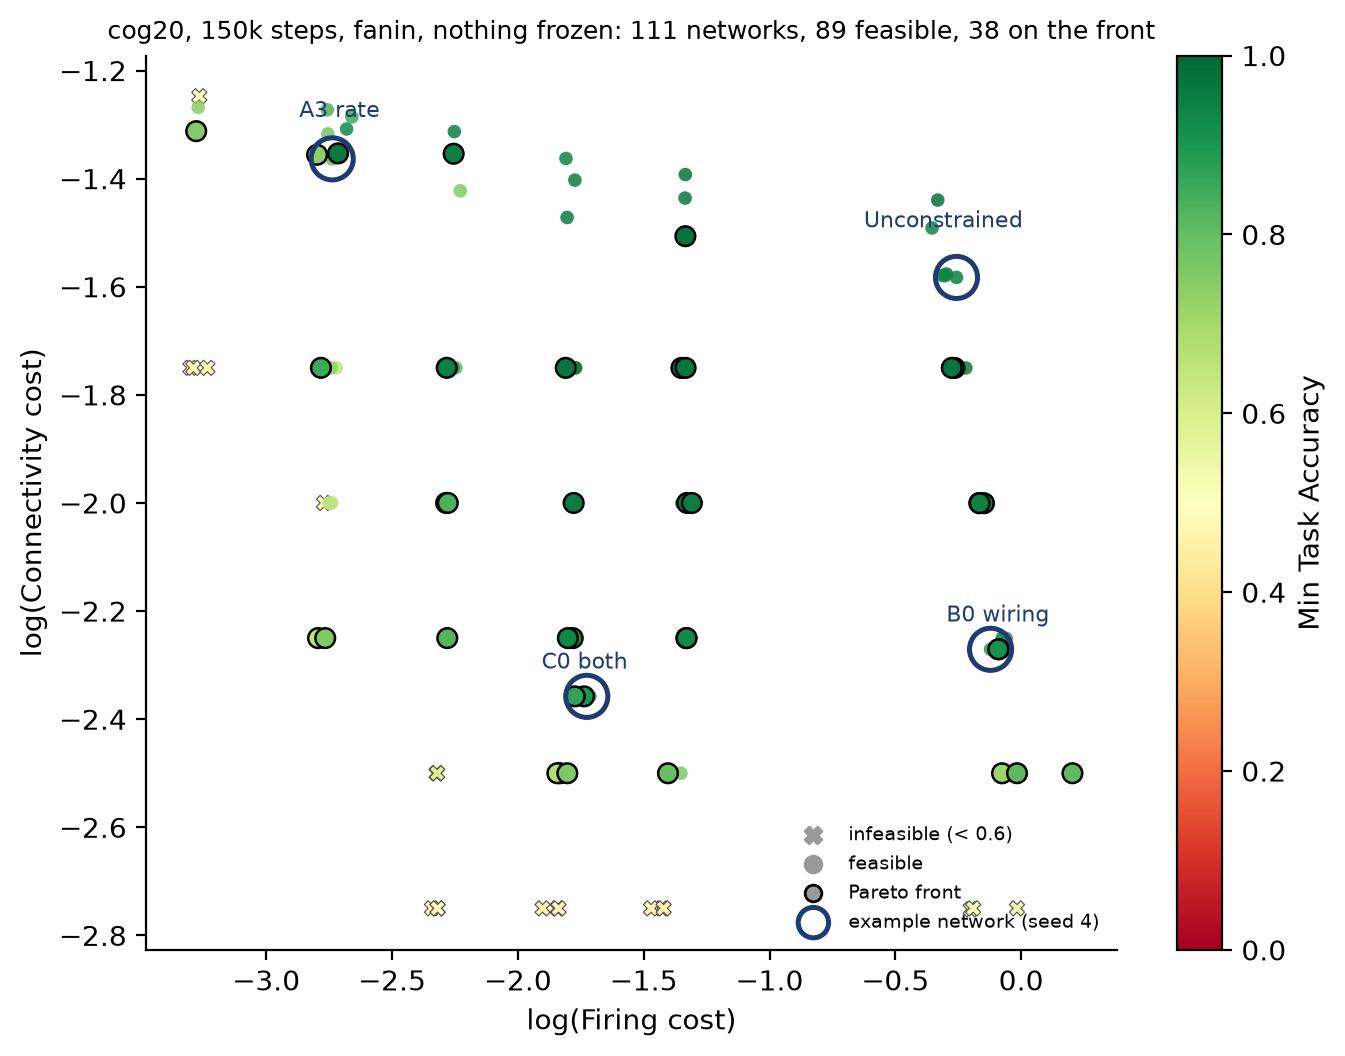
\includegraphics[width=\linewidth]{../results/front/cog20_150k_fanin_front_top.png}
    \end{column}
    \begin{column}{0.53\textwidth}
      \scriptsize
      \begin{tabular}{@{}lcccc@{}}
        \toprule
                            & control & A3     & B0     & C0     \\
                            & none    & rate   & wiring & both   \\
        \midrule
        rate budget         & --      & 0.0011 & --     & 0.0115 \\
        wiring budget       & --      & --     & 0.0054 & 0.0044 \\
        \midrule
        worst-task accuracy & 0.96    & 0.85   & 0.87   & 0.88   \\
        mean accuracy       & 0.99    & 0.98   & 0.99   & 0.98   \\
        firing cost         & 0.49    & 0.0020 & 0.81   & 0.018  \\
        wiring cost         & 0.030   & 0.047  & 0.0054 & 0.0044 \\
        synapses kept       & 70\%    & 61\%   & 6\%    & 0.7\%  \\
        \midrule
        \multicolumn{5}{@{}l}{\emph{example network (seed 4, ringed)}} \\
        worst-task accuracy & 0.95    & 0.78   & 0.89   & 0.89   \\
        \bottomrule
      \end{tabular}\\[0.8em]
      \footnotesize
      \begin{itemize}
        \item 5 seeds per point, means shown. Ringed: example network (seed 4), used from here on.
        \item A3 fires $\sim$250$\times$ less than control; B0 and C0 keep 6\% and 0.7\% of synapses.
        \item All solve the tasks: mean accuracy $>0.95$ everywhere.
      \end{itemize}
    \end{column}
  \end{columns}
\end{frame}

\begin{frame}{Do they converge?}
  \centering
  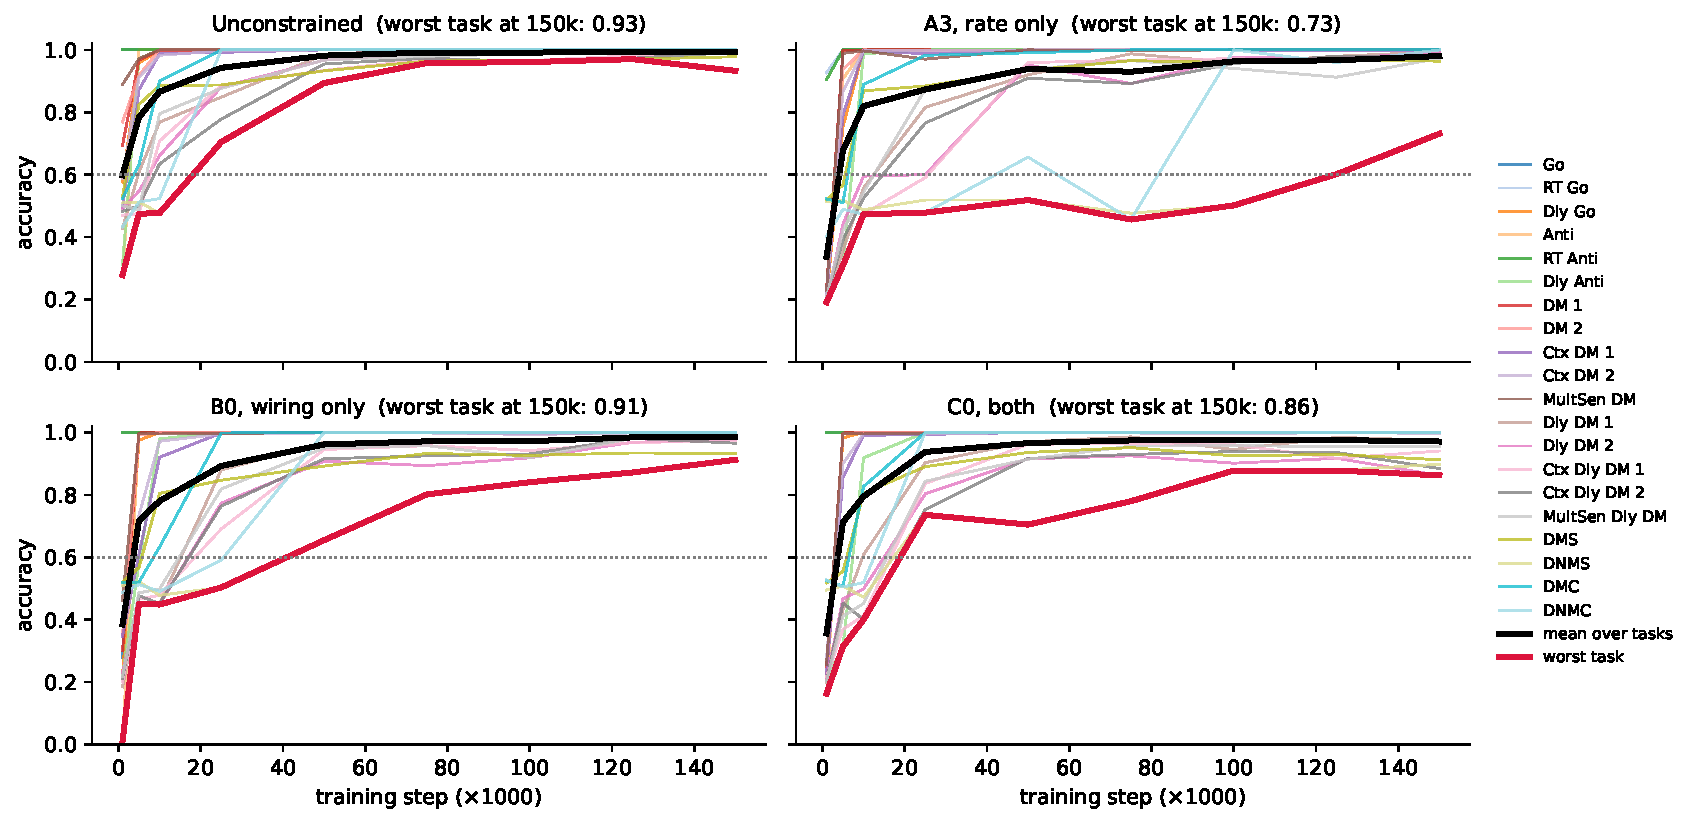
\includegraphics[width=\textwidth,height=0.8\textheight,keepaspectratio]{../results/front/acc_vs_steps_fanin_grid.pdf}\\[0.3em]
  \scriptsize Convergence checked on a separate run of the same four points (one network each, accuracy saved along
  training), not the example network.
\end{frame}

\begin{frame}{Task variance and the number of groups}
  \begin{columns}[c]
    \begin{column}{0.36\textwidth}
      \footnotesize
      \textbf{Task variance} (Yang et al.\ 2019)
      \[
        \mathrm{TV}_{i,a} = \big\langle \mathrm{Var}_{\text{trials}}\, r_i(t) \big\rangle_{t\,>\,\text{fixation}}
      \]
      neuron $i$, task $a$. Each neuron divided by its maximum over tasks: a task profile.\\[0.6em]
      \textbf{Groups}: k-means on the profiles, \textcolor{Ecol}{E} and \textcolor{Icol}{I} separately.\\[0.6em]
      \textbf{Silhouette}
      \[
        s = \frac{b - a}{\max(a, b)}
      \]
      $a$: mean distance to its own group, $b$: to the nearest other group.
      $k$ = best local maximum with $k > 2$.
    \end{column}
    \begin{column}{0.62\textwidth}
      \centering
      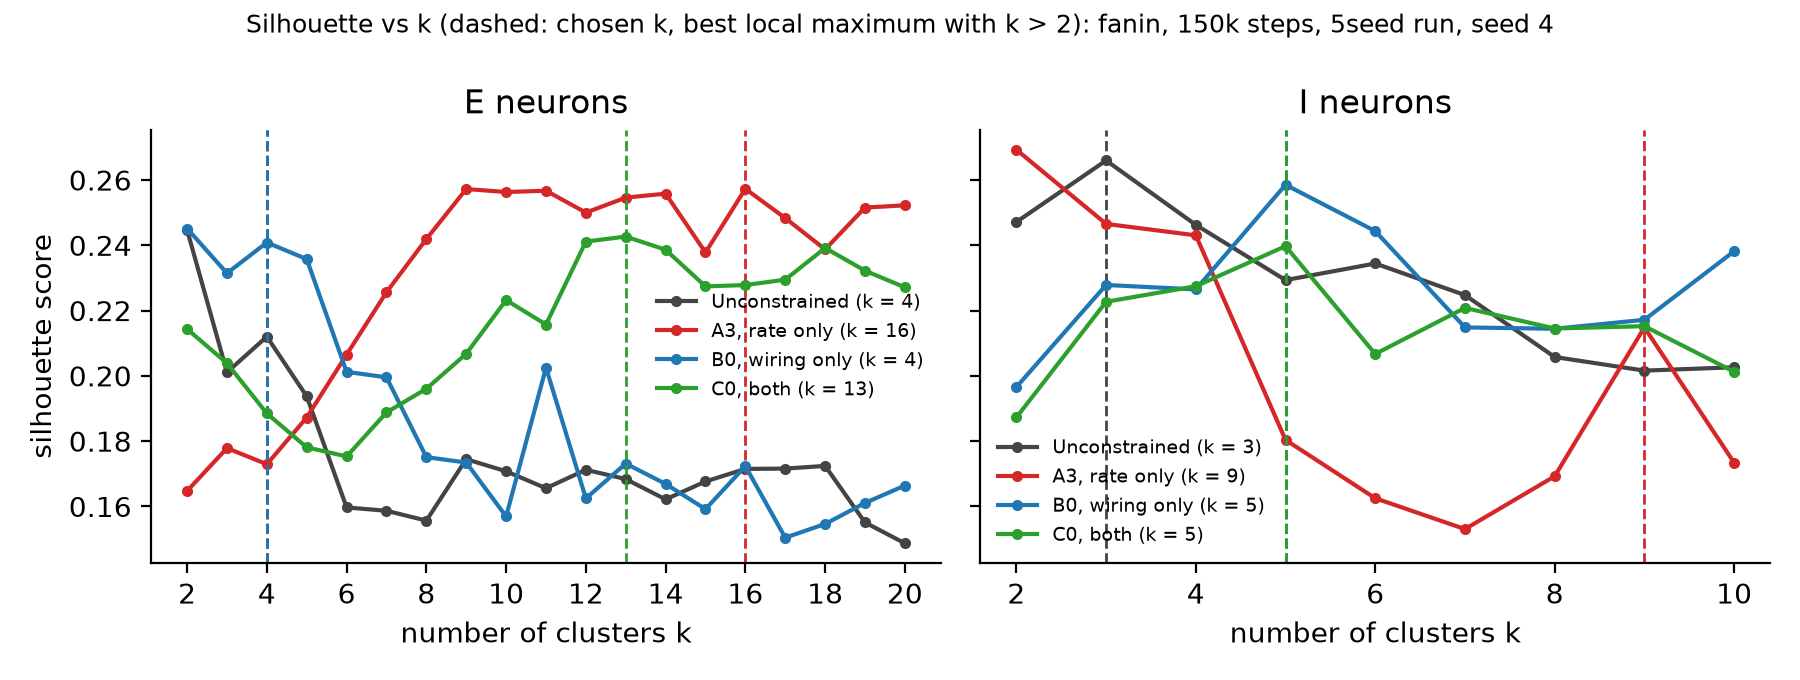
\includegraphics[width=\linewidth]{../results/front/tv_ei_fanin_5seed_s4_150k_sil.png}\\[0.4em]
      \scriptsize Silhouette vs $k$, example network (seed 4) at each point. Dashed: chosen $k$.
    \end{column}
  \end{columns}
\end{frame}

\begin{frame}{E and I groups: no budget vs.\ rate budget}
  \centering
  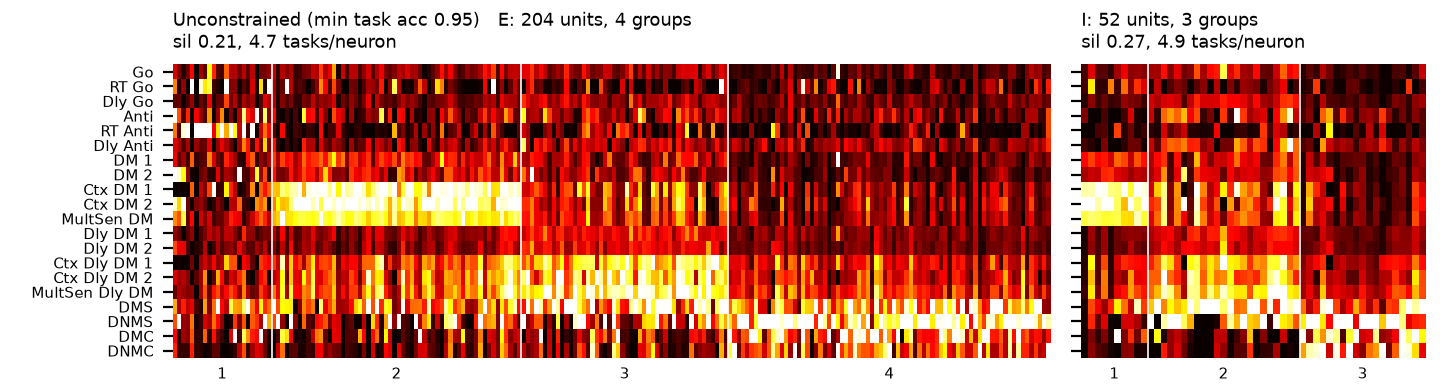
\includegraphics[height=0.4\textheight]{figs/tv_ei_control.png}\\[0.3em]
  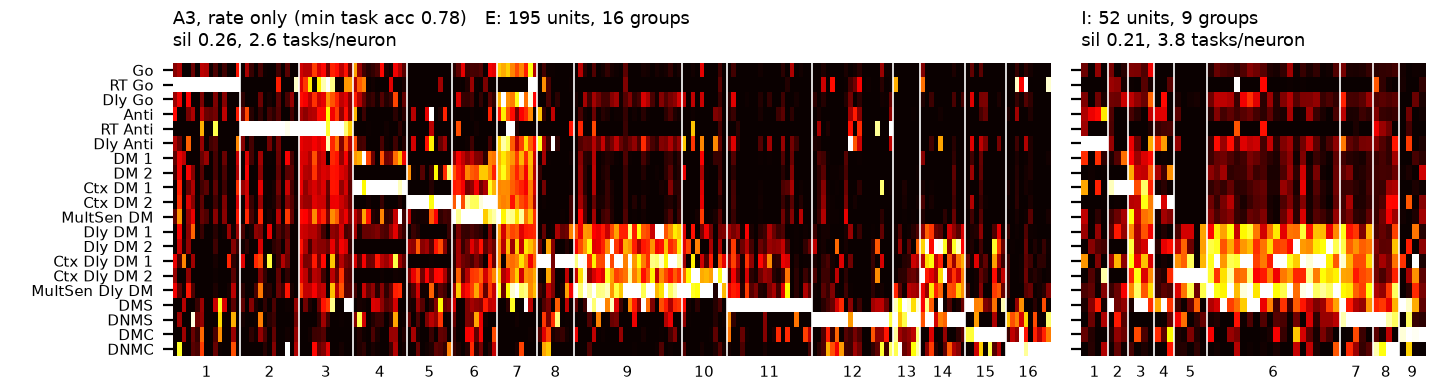
\includegraphics[height=0.4\textheight]{figs/tv_ei_A3.png}\\[0.2em]
  \scriptsize Normalised task variance (black 0, white 1); units sorted by group; left \textcolor{Ecol}{E}, right \textcolor{Icol}{I}. Example network (seed 4).
\end{frame}

\begin{frame}{E and I groups: wiring budget vs.\ both}
  \centering
  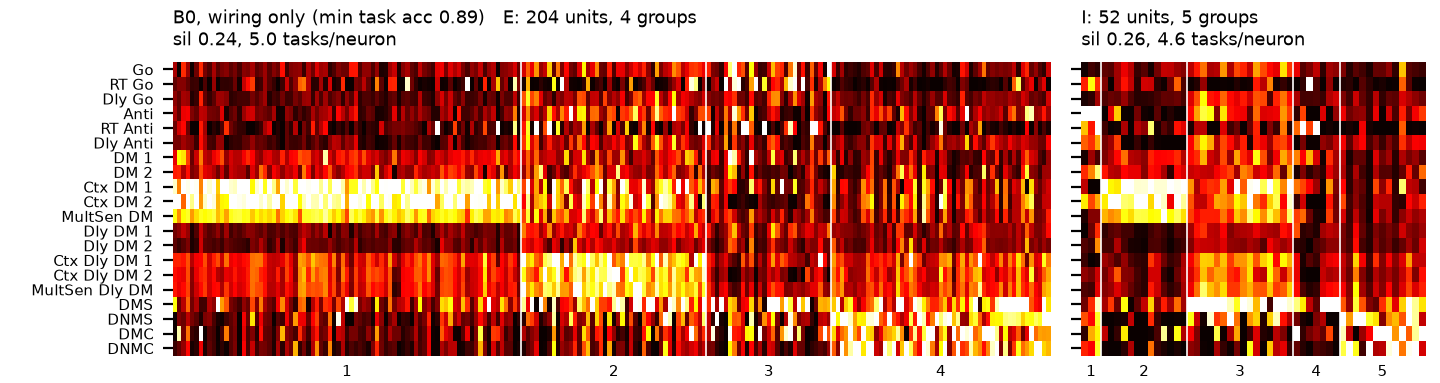
\includegraphics[height=0.4\textheight]{figs/tv_ei_B0.png}\\[0.3em]
  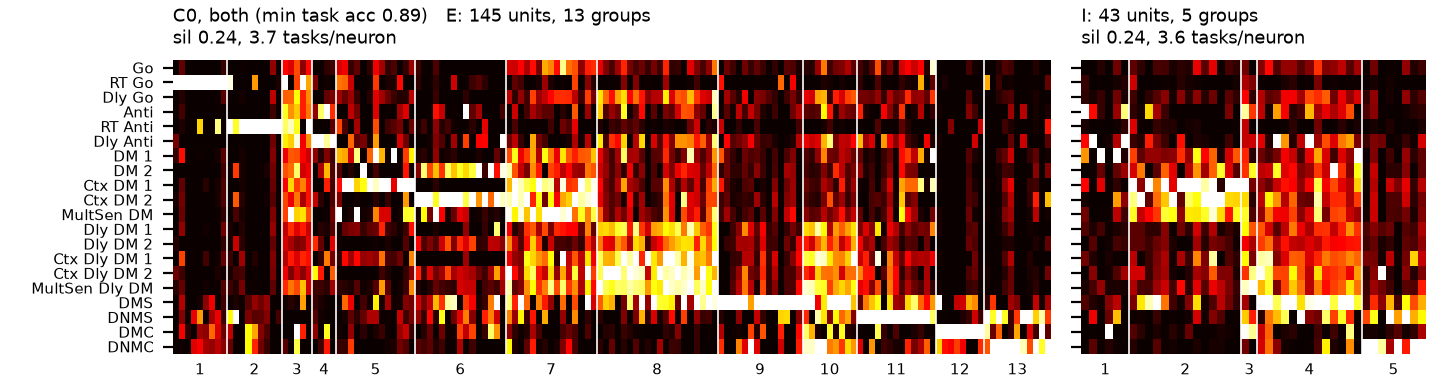
\includegraphics[height=0.4\textheight]{figs/tv_ei_C0.png}\\[0.2em]
  \scriptsize Normalised task variance (black 0, white 1); units sorted by group; left \textcolor{Ecol}{E}, right \textcolor{Icol}{I}. Example network (seed 4).
\end{frame}

\begin{frame}{Task similarity and wiring: Unconstrained}
  \centering
  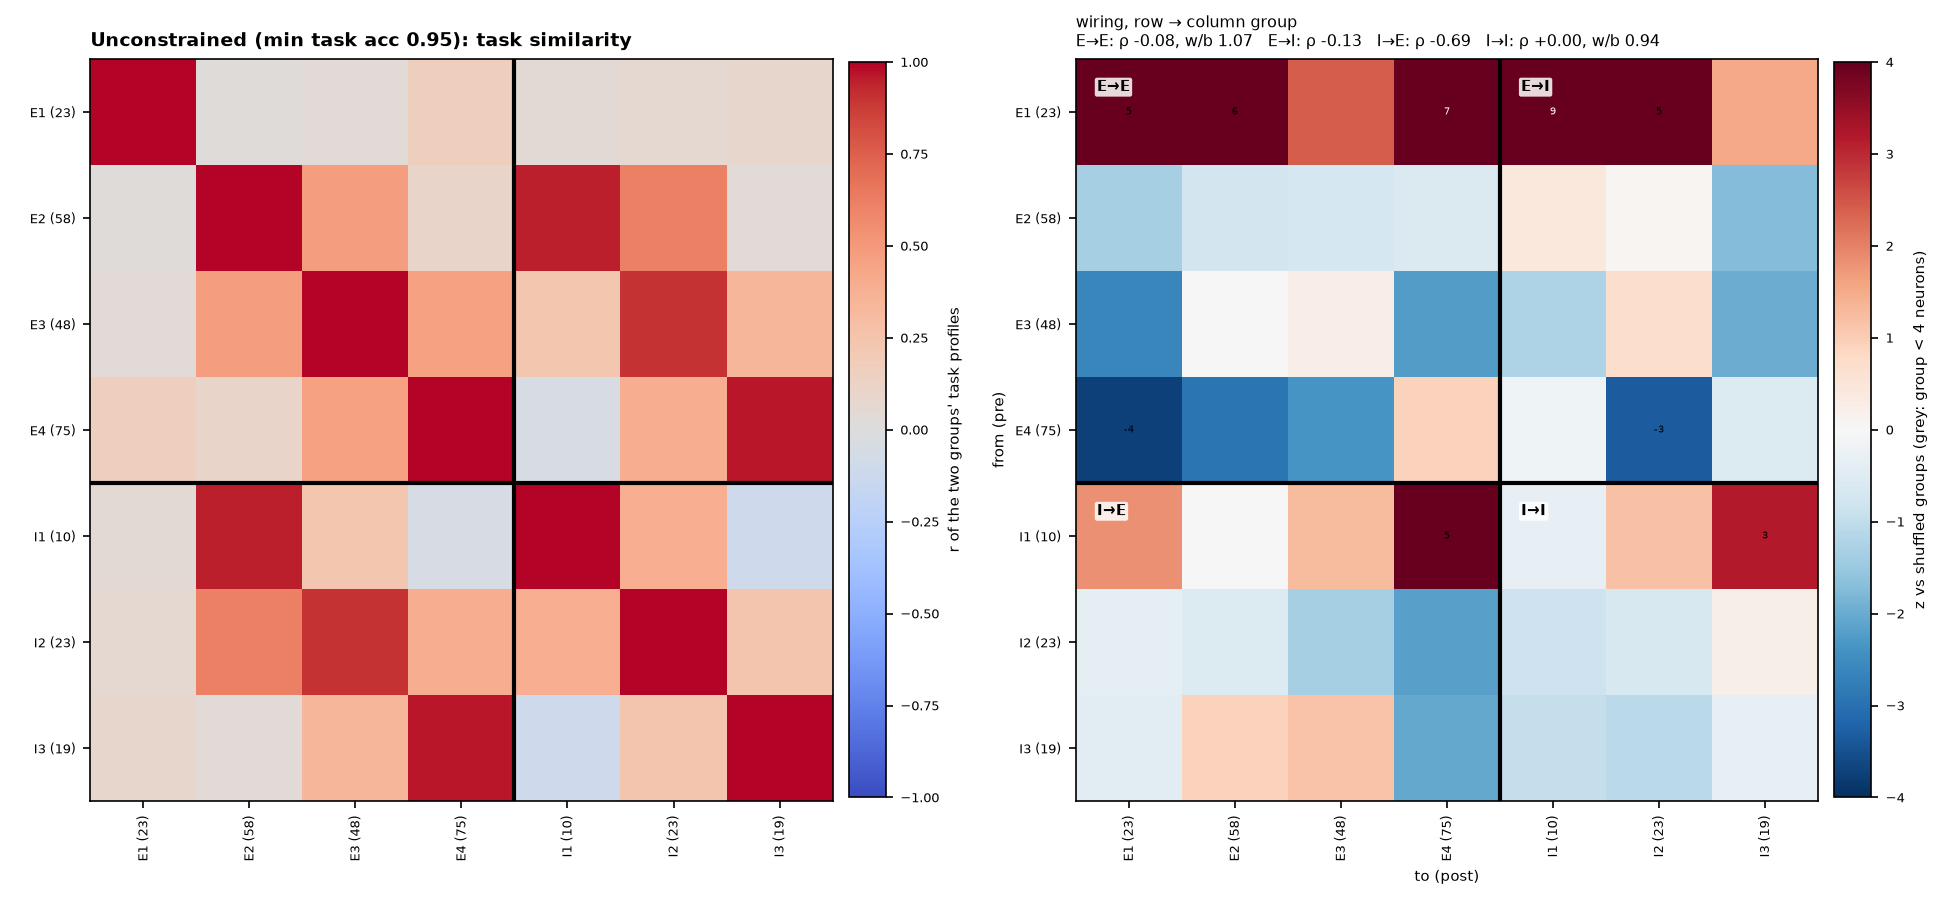
\includegraphics[width=\textwidth,height=0.74\textheight,keepaspectratio]{figs/wiring_control.png}\\[0.2em]
  \scriptsize Left: task similarity $r$ between group profiles. Right: wiring row $\to$ column group, $z$ vs 500 shuffles
  of group labels (grey: group $<4$ neurons).\\
  This network (seed 4): $\rho_{\text{I}\to\text{E}} = -0.69$, $\rho_{\text{E}\to\text{I}} = -0.13$, E$\to$E within/between 1.07. \quad All 5 seeds: $\rho_{\text{I}\to\text{E}}$ $-0.69$ to $-0.31$; $\rho_{\text{E}\to\text{I}}$ $-0.13$ to $+0.05$; E$\to$E 1.05--1.15.
\end{frame}

\begin{frame}{Task similarity and wiring: A3, rate budget}
  \centering
  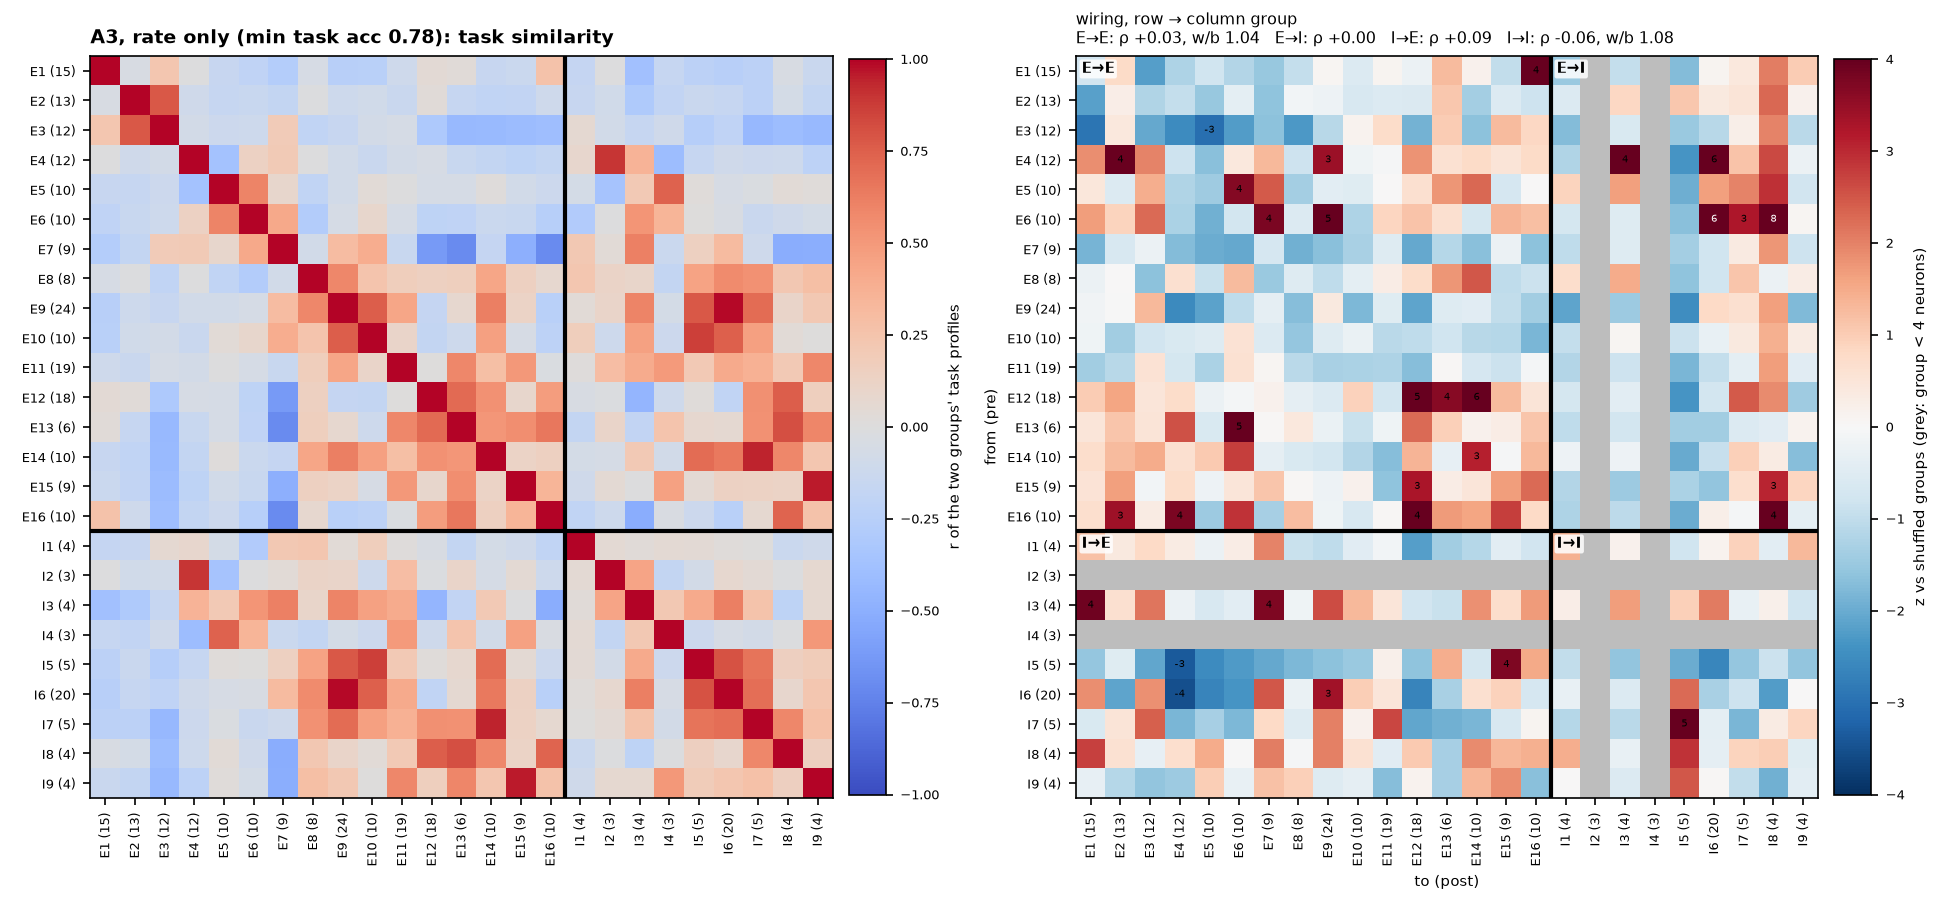
\includegraphics[width=\textwidth,height=0.74\textheight,keepaspectratio]{figs/wiring_A3.png}\\[0.2em]
  \scriptsize Left: task similarity $r$ between group profiles. Right: wiring row $\to$ column group, $z$ vs 500 shuffles
  of group labels (grey: group $<4$ neurons).\\
  This network (seed 4): $\rho_{\text{I}\to\text{E}} = +0.09$, $\rho_{\text{E}\to\text{I}} = 0.00$, E$\to$E within/between 1.04. \quad All 5 seeds: $\rho_{\text{I}\to\text{E}}$ $-0.05$ to $+0.09$; $\rho_{\text{E}\to\text{I}}$ $-0.15$ to $+0.14$; E$\to$E 1.02--1.09.
\end{frame}

\begin{frame}{Task similarity and wiring: B0, wiring budget}
  \centering
  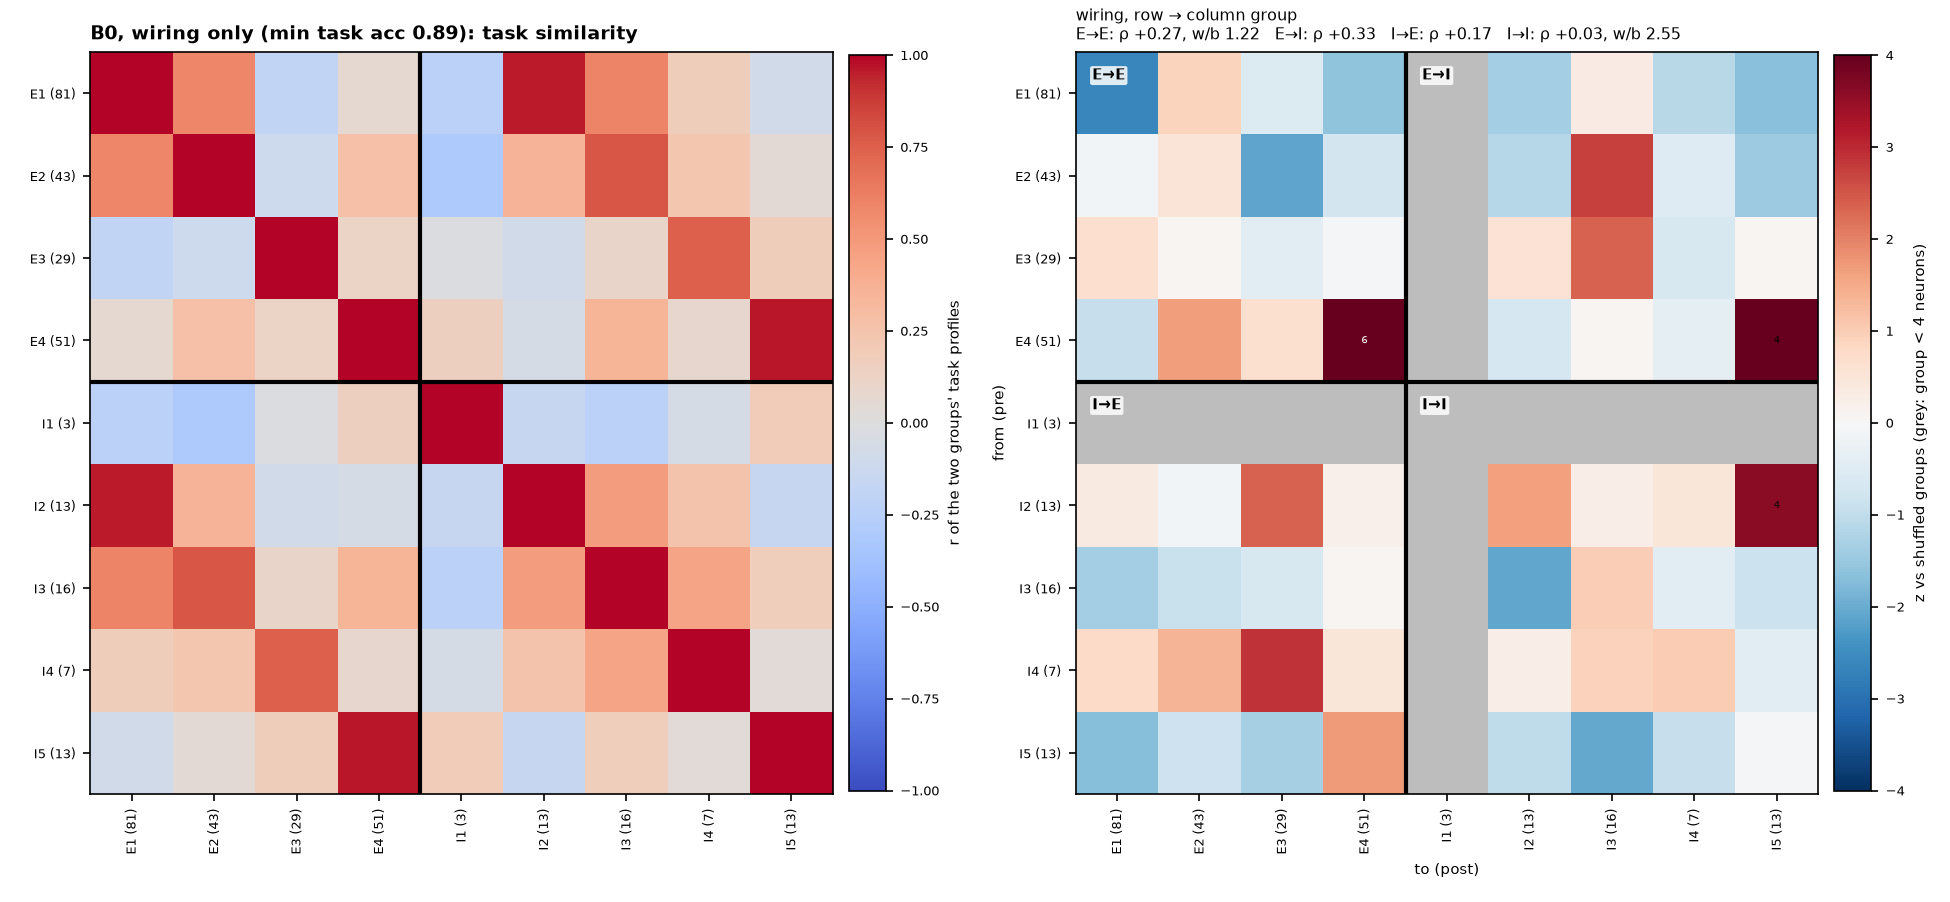
\includegraphics[width=\textwidth,height=0.74\textheight,keepaspectratio]{figs/wiring_B0.png}\\[0.2em]
  \scriptsize Left: task similarity $r$ between group profiles. Right: wiring row $\to$ column group, $z$ vs 500 shuffles
  of group labels (grey: group $<4$ neurons).\\
  This network (seed 4): $\rho_{\text{I}\to\text{E}} = +0.17$, $\rho_{\text{E}\to\text{I}} = +0.33$, E$\to$E within/between 1.22. \quad All 5 seeds: $\rho_{\text{I}\to\text{E}}$ $-0.05$ to $+0.45$; $\rho_{\text{E}\to\text{I}}$ $-0.03$ to $+0.40$; E$\to$E 1.15--5.89.
\end{frame}

\begin{frame}{Task similarity and wiring: C0, both budgets}
  \centering
  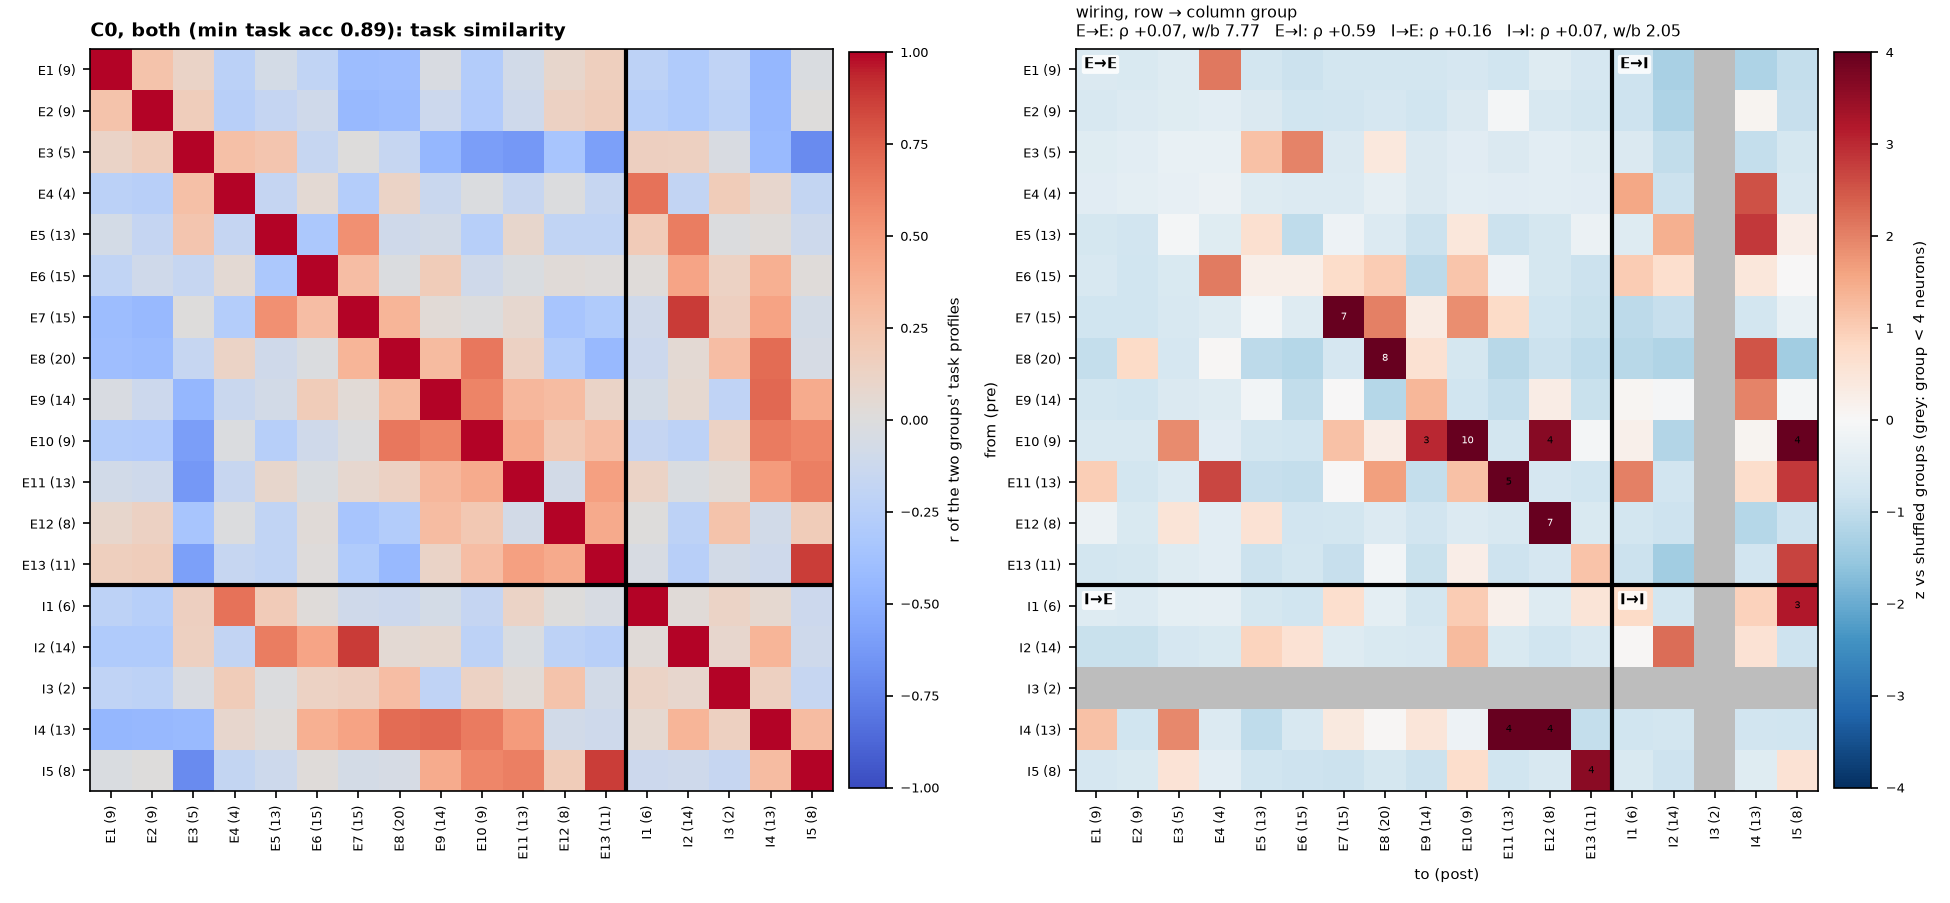
\includegraphics[width=\textwidth,height=0.74\textheight,keepaspectratio]{figs/wiring_C0.png}\\[0.2em]
  \scriptsize Left: task similarity $r$ between group profiles. Right: wiring row $\to$ column group, $z$ vs 500 shuffles
  of group labels (grey: group $<4$ neurons).\\
  This network (seed 4): $\rho_{\text{I}\to\text{E}} = +0.16$, $\rho_{\text{E}\to\text{I}} = +0.59$, E$\to$E within/between 7.77. \quad All 5 seeds: $\rho_{\text{I}\to\text{E}}$ $+0.07$ to $+0.39$; $\rho_{\text{E}\to\text{I}}$ $+0.36$ to $+0.62$; E$\to$E 2.84--7.77.
\end{frame}

\begin{frame}
  \centering\Huge Thank you
\end{frame}

\end{document}
